% Figure from MATH 591 notes, section 6. Compile with the notes preamble.
\begin{tikzpicture}[scale=1.0]
\draw[gray!45,->] (-0.3,0) -- (3.3,0); \draw[gray!45,->] (0,-0.3) -- (0,3.3);
\foreach \c/\d in {1.6/0.58, 0.7/0.26, 0.28/0.11, 0.1/0.04} {
  \draw[gray!75,domain=\d:3.1,samples=140,smooth,variable=\x] plot (\x,{\c/\x}); }
\draw[violet!75!black,very thick] (0.04,0) -- (3.1,0);
\draw[teal!60!black,very thick] (0,0.04) -- (0,3.1);
\draw[black!70, fill=white] (0,0) circle (2.2pt); \node[font=\scriptsize, anchor=north east] at (-0.04,-0.04) {$0 \notin X$};
\foreach \y in {0.7,0.28,0.1} { \fill[magenta!60!black] (1,\y) circle (1.5pt); }
\draw[gray!60,dashed] (1.08,0.72) -- (1.75,1.15);
\foreach \x in {0.7,0.28,0.1} { \fill[magenta!60!black] (\x,1) circle (1.5pt); }
\draw[gray!60,dashed] (0.75,1.06) -- (1.27,1.9);
\node[magenta!60!black,font=\footnotesize,anchor=west] at (1.27,1.97) {$\tfrac1n \cdot z_n=(\tfrac1n,1)$};
\node[magenta!60!black,font=\footnotesize,anchor=west] at (1.78,1.18) {$z_n=(1,\tfrac1n)$};
\node[violet!75!black,font=\footnotesize,anchor=north] at (2.0,-0.12) {orbit of $(1,0)$};
\node[teal!60!black,font=\footnotesize,anchor=west] at (0.12,3.2) {orbit of $(0,1)$};
\node[font=\footnotesize,anchor=north west] at (1.9,2.6) {orbits $xy=c$};
\node[font=\footnotesize] at (1.5,-0.8) {as $c\to0$ the orbit approaches \emph{both} axes};
\end{tikzpicture}
